% Specify the type of document
\documentclass[a4paper,12pt]{article}

% Load a number of useful packages
\usepackage{graphicx}
\usepackage{amsmath,amssymb,amsfonts,amsthm}
\usepackage{gensymb}
\usepackage[margin=1.0in]{geometry}
\usepackage[colorlinks=true]{hyperref}
\usepackage[caption=false,font=footnotesize]{subfig}
\usepackage[table]{xcolor}
\usepackage{biblatex}
\usepackage[utf8]{inputenc}
\usepackage{subfig}
\usepackage{textcomp}
\usepackage{amsmath}
\usepackage{float}
\usepackage[labelfont=bf]{caption}
\usepackage{setspace}
\usepackage{siunitx}
\usepackage{listings}
\usepackage[newfloat]{minted}
\usepackage{bm}
\usepackage{lscape}

\sisetup{output-exponent-marker=\ensuremath{\mathrm{e}}}

\usepackage{titlesec}
\titleformat*{\section}{\large\bfseries}
\titleformat*{\subsection}{\normalsize\bfseries}
\titleformat*{\subsubsection}{\normalsize\bfseries}
\usepackage{indentfirst}

\usepackage{fancyhdr} 
\pagestyle{fancy}
\fancyhf{}
\fancyheadoffset{0cm}
\renewcommand{\headrulewidth}{0pt} 
\renewcommand{\footrulewidth}{0pt}
\fancyhead[R]{\thepage}


\setlength{\parindent}{0.5in}
\addbibresource{references.bib}


% Two more packages that make it easy to show MATLAB code
\usepackage[T1]{fontenc}
\usepackage{mathptmx}
\usepackage[framed,numbered]{matlab-prettifier}
\lstset{
	style = Matlab-editor,
	basicstyle=\mlttfamily\small,
}

% Say where pictures (if any) will be placed
\graphicspath{{./pictures/}}

% Define title and author (date is auto-generated, unless you define it)
\usepackage{xurl}

\begin{document}

% Title
\begin{center}
    \Large\textbf{ECE 470: Final Project Report}
\end{center}
\begin{flushright}
	Team: Charlie Ray, Kenneth Tochihara, Jeffery Zhou \\
	TA: Dhurv Mathur \\
	Section: Monday 9AM \\
	Team Name: GouBot
\end{flushright}

% Report Body
\section{Team and Links}\label{sec:introduction}
    \noindent The following are the team members of GouBot and their respective NetIDs.
    \begin{itemize} 
        \item Jeffery Zhou: shijunz2
        \item Kenneth Tochihara: ktt2
        \item Charlie Ray: cfray2
    \end{itemize}

    \noindent The following are the GitHub link and YouTube link to the final video. 
    \begin{itemize}
    \allowbreak
        \item GitHub: \href{https://github.com/ktt3/ae482_goubot}{Link}
        \item YouTube Final Demonstration: \href{https://www.youtube.com/watch?v=X16YSidoG5w&list=PLUgYn1EdVdaukTL5irfwSSML7CPnV4CY7&index=3}{Link}
        \item YouTube Playlist: \href{https://www.youtube.com/playlist?list=PLUgYn1EdVdaukTL5irfwSSML7CPnV4CY7}{Link}
    \end{itemize}

\newpage
\section{Introduction} \label{sec:intro}
    
    % Provide brief motivation for your pick and place application, conveying why this is an important (or fun) task. Also provide a brief summary of the approaches you used.

    After viewing some of the past projects conducted by students in this class, the GouBot team decided that although those projects were innovative and addressed real-life applications, few addressed the issues of bringing happiness to the users. The team realized the innate challenge of pick and place applications lay in the creative design of its applications. The team emphasized the happiness of the users and treated as the number one priority when coming up with the conceptual design of the robot. Knowing that dogs have been human's companion and friends for centuries, the team decided to make a robot that could play fetch with its owner so that it could bring some level of happiness to the user in an environment where pets are not allowed. The team strongly believed that such a robot would be a popular purchase for college students since few college town apartments allow pets. 

    With the motivation described above in mind, the team decided to incorporate the familiar UR3 robot with a cart robot so that the combined system could have a high level of maneuverability and flexibility to play fetch with the user. With the background provided in the lab section of the ECE 470 class, the team would be able to extract the useful functions and capabilities of the UR3 robot to perform simple pick and place actions. Knowing that the core function of fetching or picking would not be too difficult, the team decided to focus its efforts in the integration between the differential drive robot and the existing UR3 architecture. The team used Gazebo as the simulation environment and Robot Operating System (ROS) to control the robot \cite{ros_concept}. This requires knowledge about the workings of the \lstinline!.xacro! files of the major physical components and the \lstinline!.launch! files since they serve as the junction between various different architectures in Gazebo. It also requires the knowledge of how ROS works with the Gazebo environment and how to control the robot through the environment.

\newpage
\section{Task Description} \label{sec:task_desc}
    
    % Give a detailed description of your task and robot pipeline. Include specifications and design choices you made to make the task easier. Provide a block diagram that shows the different components of your system (e.g., perception/sensing, planning, grasping/picking). Describe how you implemented all of the different components in your system (e.g., how did you model your system? how did you implement inverse kinematics? what planner did you use?). If you built off of existing codebases, please give credit to the original authors.
    
    % Logic Description
    \subsection{Logic Description}
    
        The overall goal for this robot is to travel bring back the block at a randomly spawned location of the block. The robot consists of the UR3 robot mounted on a cart that can move around the environment, simulating the mobile component of a dog. The end-effector tool on the UR3 was kept as the gripper to increase the level of integration with the kinematics. To mitigate the ease of use with the transformations required for these tasks, the robot moved through translations, which made the execution of these tasks simpler due to lack of need to do rotation matricies. Though it may not be as efficient, it increase the ease of implementation for this project. The following is the general order of operations for the robot. The cart was moved to the location offset by the specified value to account for block collision of the robot. Figure \ref{fig:pipeline} describes the translation of information to action of the robot. 
        
        \begin{enumerate}
            \item Randomly generate block location
            \item Sense block location
            \item Move to the block location offset by x = -0.5 m
            \item Pick up the block
            \item Move back to spawn location of the robot
            \item Place block in front of the robot
        \end{enumerate}
        
        \begin{figure}[h]
        	\begin{center}
        	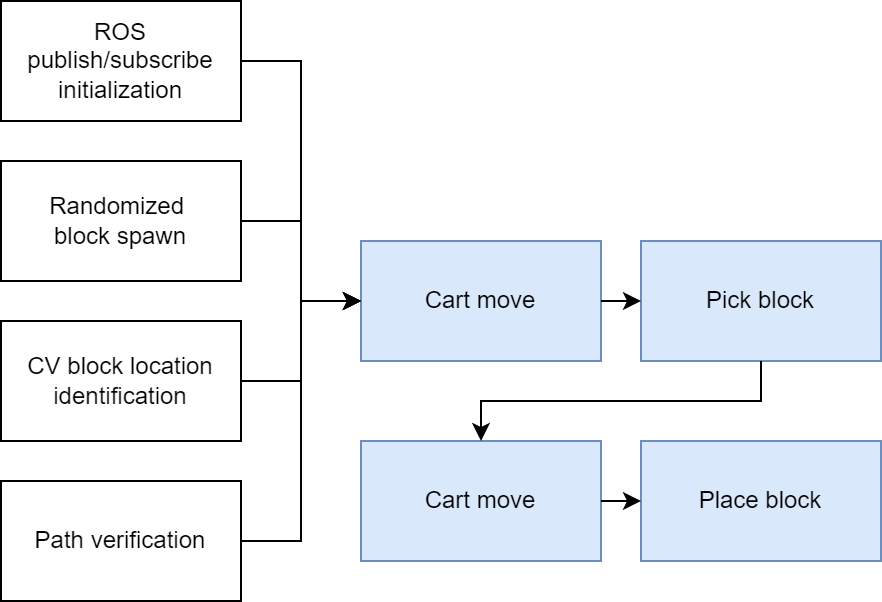
\includegraphics[width=0.8\textwidth]{pictures/information piplien.drawio.png}
        	\caption{\textbf{Information Pipeline}}
        	\label{fig:pipeline}
        	\end{center}
        \end{figure}        
        
        
    
    % Perception and controls
    \subsection{Perception and Controls}
        
        For this robot, two main modes of perception were used. The first method was the gripper input. This gripper is the same one utilized in the labs for ECE 470, where a gripping command can be sent to the gripper itself, but also responds as a sensor where it tells the user if the gripper is gripping. Computer vision was also used in the perception of the world for the robot. Though the team still utilized the same camera from the lab simulations, the location was changed to increase the ease of implementation. The camera was moved above the origin of the world coordinates, and the camera was moved higher to increase thee task space of the robot. 
        
        To control the robot, two separate controllers were used. One to move the UR3 arm, and one to move the cart itself. The execution file handles both controllers to controller the overall robot. Running the pick and place commands through the existing UR3 controller, and the cart move commands through the cart controller. Figure \ref{fig:block_diagram} represents the ROS perception and controls diagram through the \lstinline!rqt_graph! tool provided to visualize the interactions between components in the overall system \cite{ros_concept}. 
        
        \begin{figure}[h]
        	\begin{center}
        	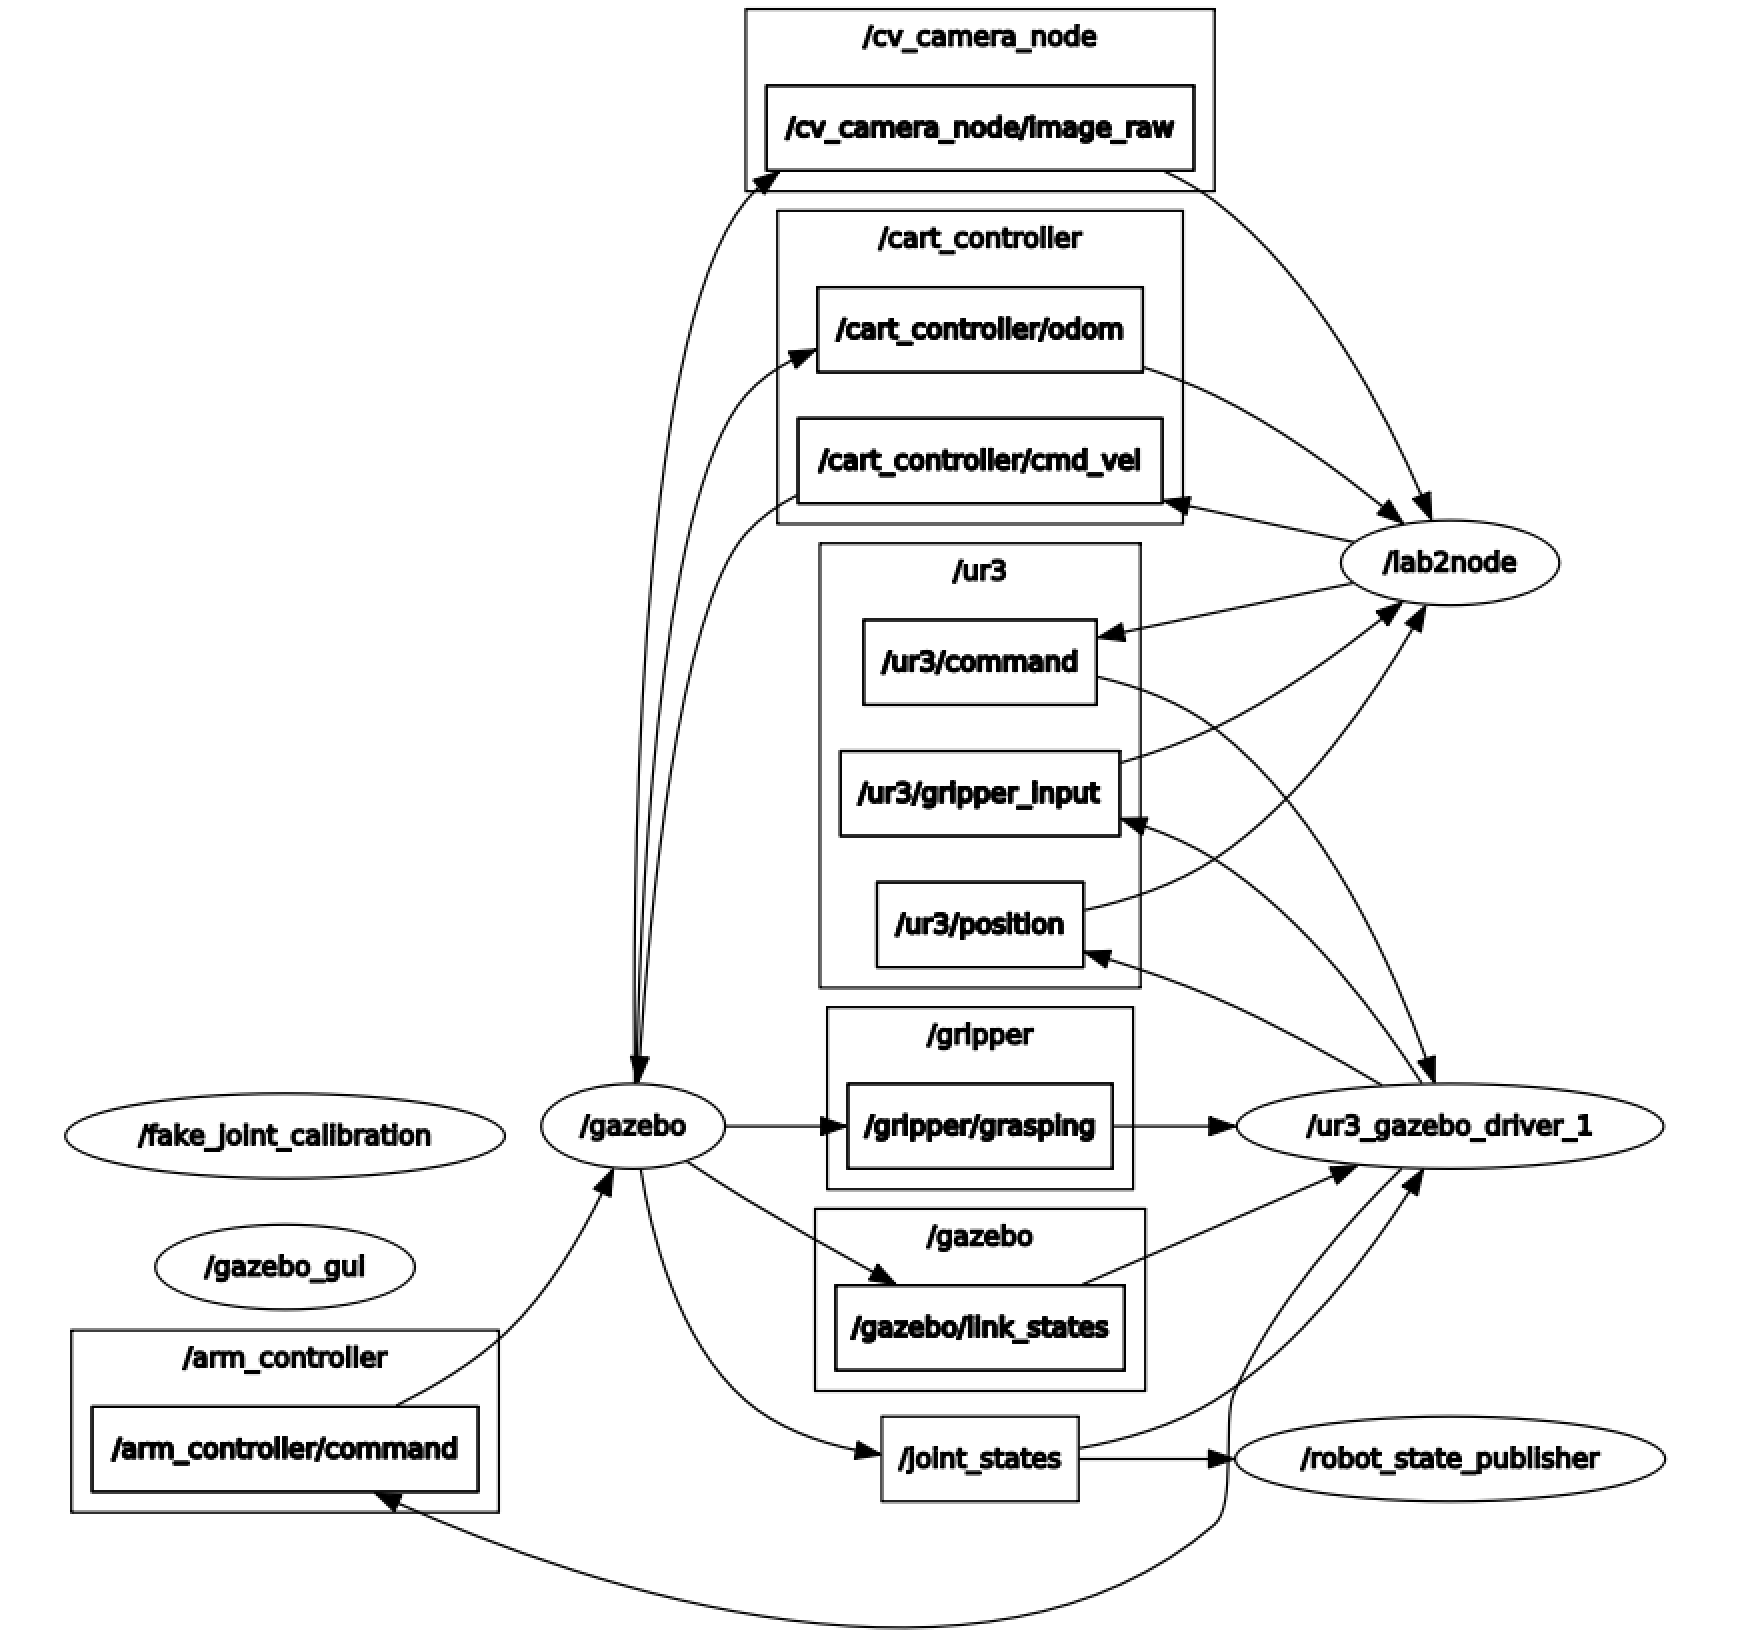
\includegraphics[width=0.8\textwidth]{pictures/block_diagram.png}
        	\caption{\textbf{GouBot Interface Diagram}}
        	\label{fig:block_diagram}
        	\end{center}
        \end{figure}
    
    % Implementation
    \subsection{Implementation}
    
        % Model description, and controller decision
        The system was modeled using the URDF files. The main task for this project was to understand the existing UR3 architecture and integrate a cart controller with it to create GouBot. Initially a differential drive controller was used as the repository for this cart already existed with the appropriate control interfaces already implemented \cite{diff_drive_robot}. However, due to the complexity of the physics simulation of the robot, the implementation was not successful. The cart was properly integrated with the UR3, but the cart would not move accurately to what velocity vectors were published. Instead, the team used a simpler controller, the planar move controller \cite{planar_move_controller}. Though this was less realistic in its application, this Gazebo plugin performed much more accurately and allowed the team to control the location of the robot arm more effectively. 
        
        % figure about the differential drive robot
        \begin{figure}[h]
        	\begin{center}
        	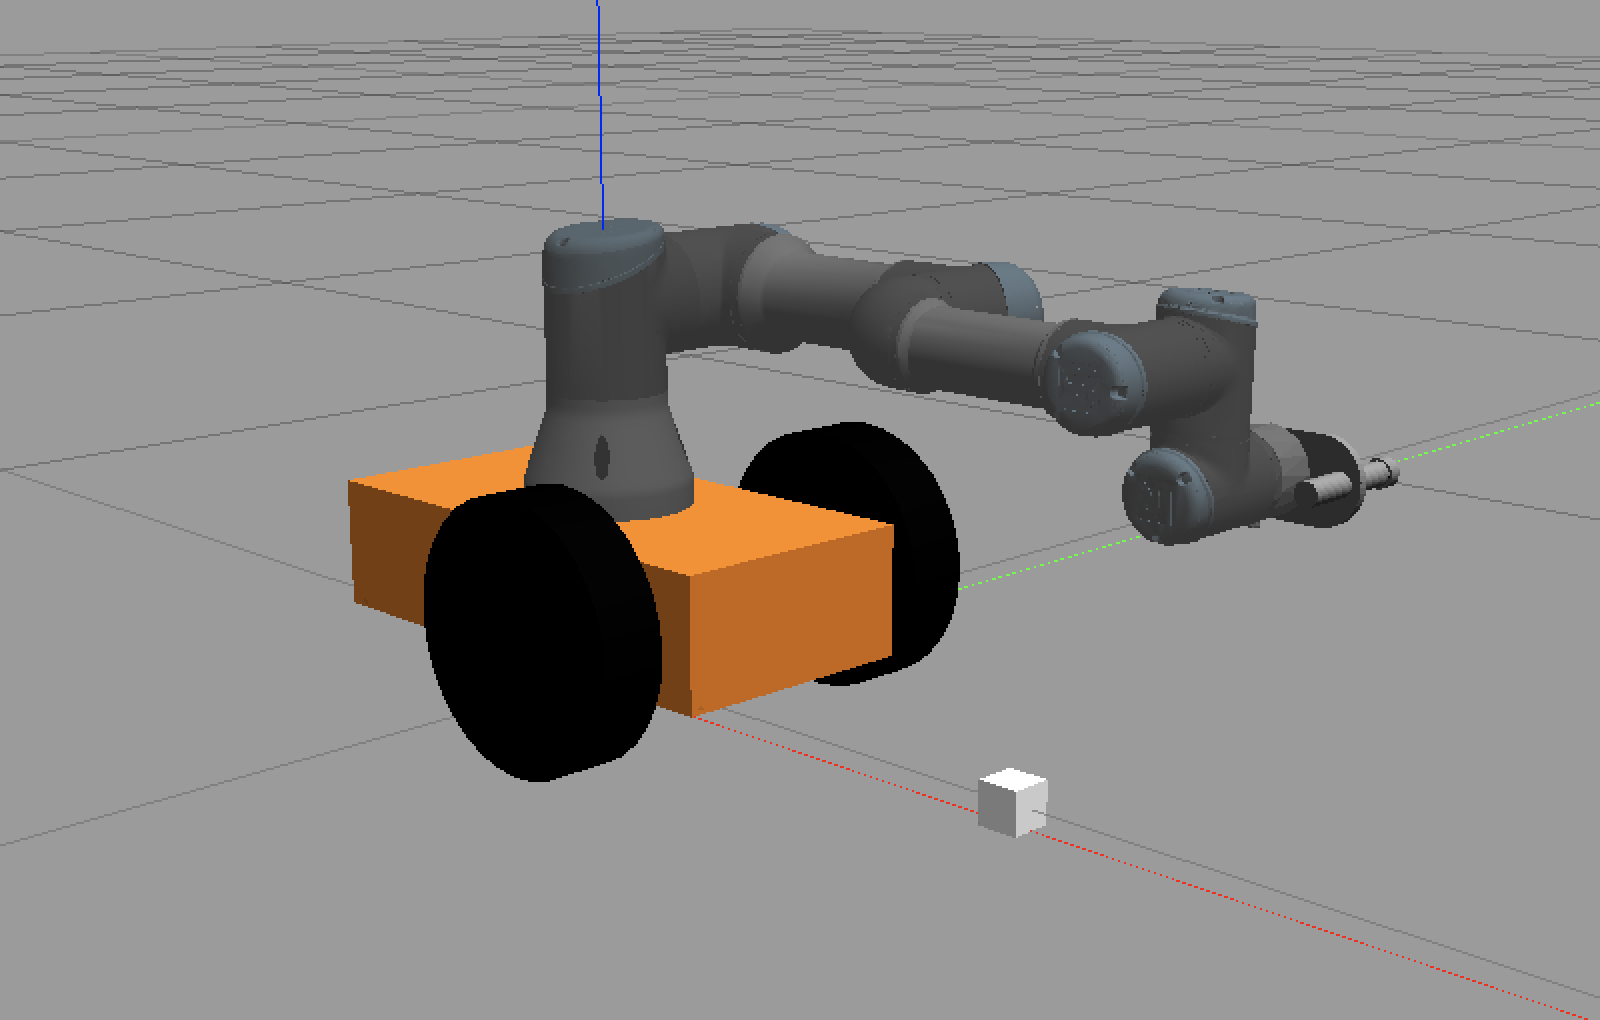
\includegraphics[width=0.55\textwidth]{pictures/diff_drive.png}
        	\caption{\textbf{Robotic Arm with Differential Drive Robot}}
        	\label{differential_drive_robot}
        	\end{center}
        \end{figure}
        
        % figure about the planar move robot
        \begin{figure}[h]
        	\begin{center}
        	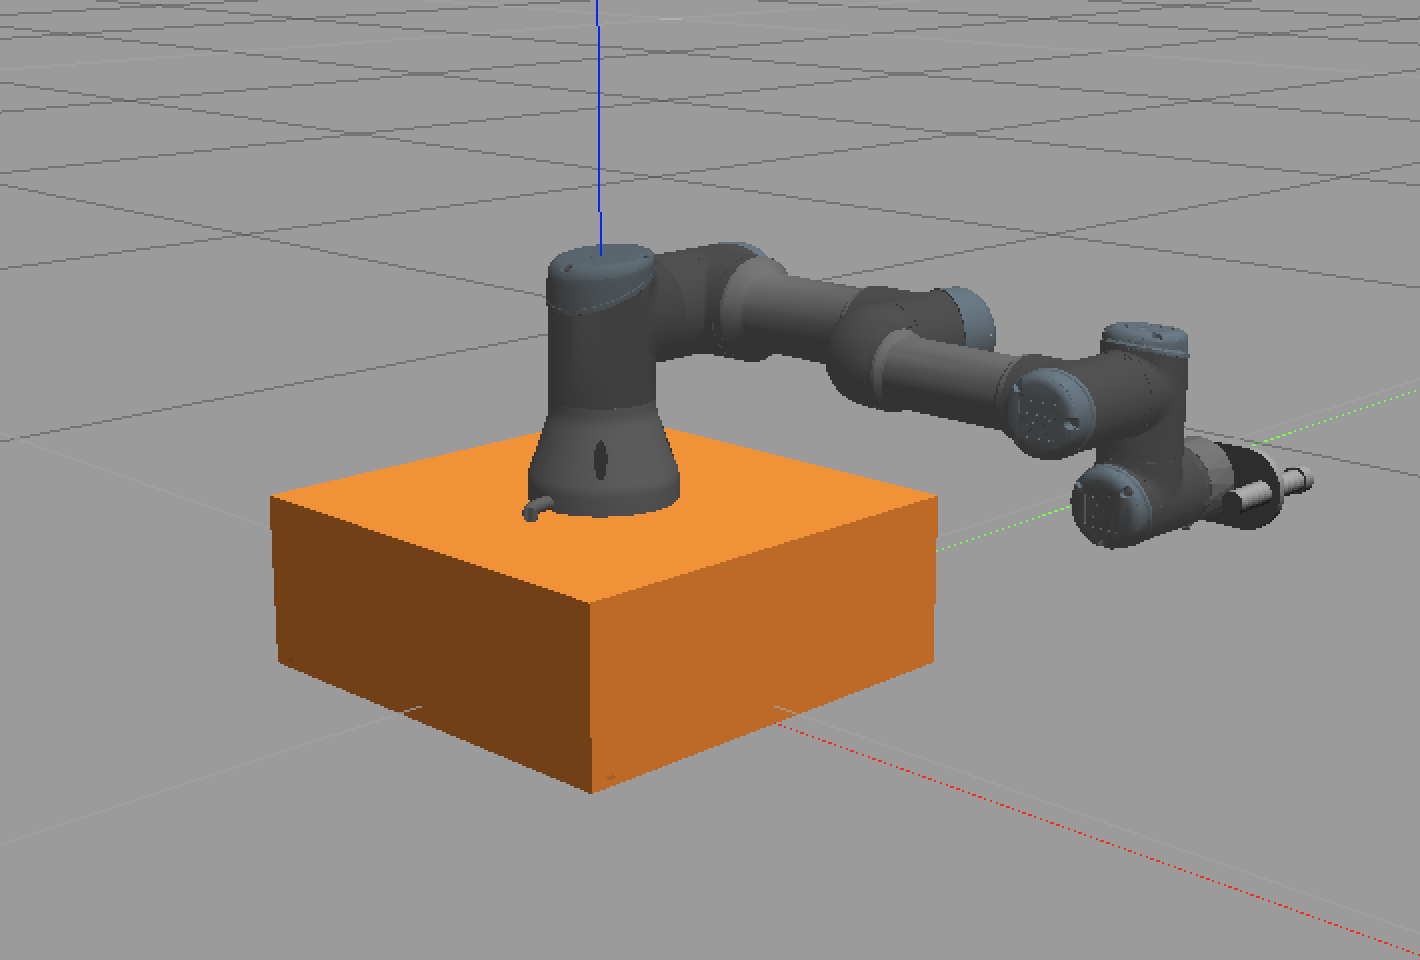
\includegraphics[width=0.55\textwidth]{pictures/planar_prism.png}
        	\caption{\textbf{Robotic Arm with Prismatic Base}}
        	\label{prismatic_robot}
        	\end{center}
        \end{figure}
        
        % end-effector dynamics
        Once the cart was properly implemented, the focus turned towards the kinematics of the robot. In comparison to the task space of the UR3 used in lab, this application required significantly more involved transformations to appropriately locate the end-effector tool in the world coordinate system. The main base frame for this robot is located at the center block of the chassis, so accounting for this offset, the proper spawn offset was utilized such that the UR3 spawns on top of the chassis. Furthermore, the base of the chassis was transformed to account for the z-axis offset from the spawn point. Figure \ref{fig:robotic_frame} describes the different frames used to calculate the dynamics of the end-effector.
        
        % include frames used in the robot
        \begin{figure}[h]
        	\begin{center}
        	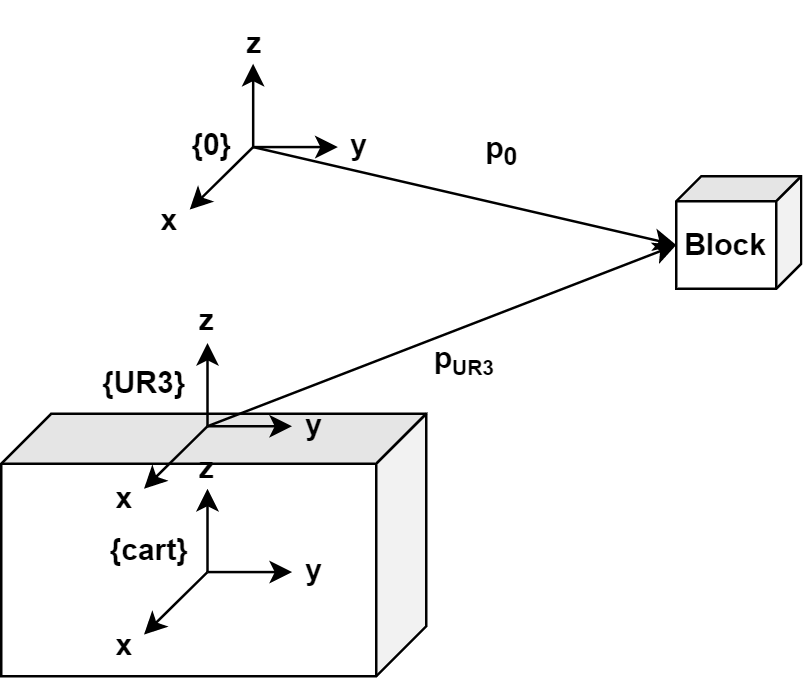
\includegraphics[width=0.75\textwidth]{pictures/transforms.png}
        	\caption{\textbf{Coordinate Systems In GouBot}}
        	\label{fig:robotic_frame}
        	\end{center}
        \end{figure}
        
        % talk about the transformations
        To calculate the kinematics of the end-effector tool. Multiple transformations were applied using information on the \lstinline!cart_controller\odom! topic, which represented the offset transformation from the original spawn point of the robot. Given that the robot cart was spawned at the origin of the world coordinates, this published value represented the transformation from the world frame to the cart frame. Furthermore, given the location of the block in the world coordinates, that value needed to be transformed to the frame of the base of the UR3 robot. Therefore, using Equation \ref{eqn:transform}, the transformations were applied the block location to generate the kinematics for the block location to use in the modified code for the forward and inverse kinematics of the robot. The transformation from the world coordinate to the UR3 ($T_{0,\text{UR3}}$) were calculated, and the inverse of the transformation ($T_{0,\text{UR3}}^{-1} = T_{\text{UR3}, 0}$) was take to convert the position of the block in the world frame ($p_0$) to the UR3 frame ($p_{\text{UR3}}$). This value is given to the inverse kinematics function in \lstinline!lab2_func.py!.
        
        % equation for the transformations
        \begin{equation}
            \label{eqn:transform}
            p_{\text{UR3}} = (T_{0,\text{cart}}~T_{\text{cart},\text{UR3}} )^{-1}p_0
        \end{equation}
        
        % talk about the offset move
        To make the pick and place maneuvers simpler, \lstinline!cart_controller\cmd_vel! was used to move the robot to the offset value of the location of the block. If the robot moved to the actual location of the block, the robot would collide with the block. Therefore, this offset was implemented to ensure collision avoidance. In this application, the robot was 0.5 m in front of the block, making the pick and place simple for the robot. However, to ensure the highest accuracy, the robot still used the transformations using the coordinates of the block and pose of the cart to determine the exact joint angles to pick and place the blocks. Even though the computation of the UR3 dynamics would be simplified using the given static offset from the block that the cart moves to, there could still be error build up from the cart location. This informed the team's design to calculate the kinematics of the UR3 arm using the actual world coordinates of the block and the transformation of cart instead. 

\newpage
\section{Experimental Setup} \label{sec:experimental_setup}
    
    % Carefully describe your simulator setup, both in terms of the environment design and the robot. Summarize how you generated scenarios to test and gather results (e.g., did you randomly generate blocks to be sorted? how did you control for difficulty).
    
    % simulation setup
    \subsection{Simulation}
    
        There were two major components of the simulation that needed to be set up for this project: the robot and the environment. The team decided not to modify the environment since it has been set up to have everything the team needs. The robot's goal was to locate and retrieve a randomly generated object, so there were a few important functionalities that it needed to provide. There needed to be an arm that could pick up the object, a vehicle to transport the arm to and from the object, and an object to pick up. Additionally, a camera was needed to locate the object and provide the location and orientation of the block to GouBot.
    
        To understand how the arm was simulated, it was essential to investigate the main architecture of the UR3 and how it all fits within the framework of the Gazebo software system. The sections below demonstrate how each component of the GouBot fits together and forms a cohesive unit in Gazebo simulation. This architecture will be divided into three different levels and where each smaller numerical level is housed within one with a higher numerical level. 
        
        \subsubsection*{Level 1: URDF Descriptions}
            
            Level 1 houses each of the individual \lstinline!xacro! files for the two component of the final GouBot which are the UR3 robotic arm and the cart itself. Under the \lstinline!universal-robot/urdf! path, \lstinline!ur3.urdf.xacro! and \lstinline!myrobot.xacro! can be found \cite{diff_drive_robot}. They represent the physical description of the UR3 robotic arm and the cart including the inertial and visual components. These files are represented as individual robots, and can work independently from one another.
            
        \subsubsection*{Level 2: Robot Integration}
                
            Level 2 houses the integrated \lstinline!xacro! files in \lstinline!ur3_robot.urdf.xacro! and has both robots imported together to create one larger robot. Given the nature of common \lstinline!xacro! architecture, a specific joint has to be made and defined that joins the UR3 robotic arm and the cart together. A fixed joint was made to join the parent link, the cart, and the child link, the UR3 robotic arm. Specifically, the fixed joint is located at a specific location as shown in the equation below so that the two joints can be correctly joined together.
        
        \subsubsection*{Level 3: Launching Environment}
            
            Level 3 houses the two different launch files and each has a different purpose. The first launch file  \lstinline!ur3.upload.launch! incorporates the previously combined \lstinline!xacro! file so that later on it could be called in the second launch file to be launched into the Gazebo world. The second launch file is the Gazebo launch script \lstinline!ur3.gazebo.launch! and it includes the model launch file mentioned in addition to the world file, additional controllers for the robots, and everything else that are essential for the simulation world. 
    
            Now, the Gazebo world should be able to successfully spawn the GouBot consisting of both the UR3 robotic arm and the cart as shown in Figure \ref{differential_drive_robot} down below. The robot is spawned exactly at the origin of the world frame. 
    
        \subsubsection*{Cart Control}
    
            In order to move the robot arm to the object and perform the fetching function, a prismatic block was attached to the base joint of the UR3 robot. This required the team to edit the existing \lstinline!.xacro! files by adding a \lstinline!.urdf! of the block and fixing it onto the bottom of the robot. To move the robot, two arguments are needed. First, the program recognizes the destination of the block in the body frame of the robot which consists of $[x,y]$. Then, the user could define a velocity magnitude of which the robot will move. In this case, the robot would be able to move to any position in the gazebo world with a specific velocity.
        
        \subsubsection*{Camera}
        
            The camera is an equally important component of the simulation. It is the robot's only source of perception that can locate where a block has spawned. It does so using OpenCV's blob detection functionality which can recognize a region of similarly colored pixels that are different from the surrounding pixels. The \lstinline!blob_search()! function that was created in lab was repurposed to identify the white blocks against Gazebo's default dark gray background. One tedious yet important step of using a camera is the calibration. The team found an easy solution that simplified the calibration process. The camera was moved above the origin of Gazebo world frame. This step automatically removes the $T_x$ and $T_y$ values from the calibration step. Subsequently by placing the block at $[1,0,0]$, the beta value could be obtained by using the pixel displacement form the origin to the above mentioned location and dividing the two quantities. Once the calibration coefficients were determined, the GouBot have all the right functionalities to perform the fetching task the team designed it for. 
    
    % Testing environment
    \subsection{Testing}

        To test the robot's capabilities the team chose to use small blocks, similar to the colored blocks used in lab, because they were easy to model, spawn, and manipulate in simulation. The coordinates for these blocks are randomly generated using the function \lstinline!block_spawn_location()! which is located in \lstinline!lab2_func.py! \lstinline!block_spawn_location()! and it works by using Numpy's random generation functionality to generate four parameters: \lstinline!n_valx!, \lstinline!n_valy!, \lstinline!n_signx!, and \lstinline!n_signy!. In addition, the team defined the task space for the GouBot, spawning only within the viewable area of the camera, while also not allowing for block spawns inside the robot. This is reflected in the code snippets shown below: 
    
        \begin{quote}
            \begin{lstlisting}[gobble=12,language=python]
            # define spawn range
            x_width_outer = 1.25; x_width_inner = 0.3
            y_width_outer = 1.75; y_width_inner = 0.3
            # generate random values for calculation
            n_valx = np.random.rand(); n_valy = np.random.rand(); 
            n_signx = np.random.rand(); n_signy = np.random.rand(); 
            \end{lstlisting}
        \end{quote}
        
        These parameters each correspond to the values of the x- and y- coordinates, and their sign - that is, whether they are positive or negative. The values are scaled so that they fall within the bounding box defined above and the signs are applied before the final values are returned.
        
        \begin{quote}
            \begin{lstlisting}[gobble=12,language=python]
            # generate random coordinates
            x = ((x_width_outer - x_width_inner)* n_valx + x_width_inner) *
            ((n_signx - 0.5)/abs(n_signx - 0.5))
            y = (y_width_outer * n_valy)*((n_signy - 0.5)/abs(n_signy - 0.5))
            \end{lstlisting}
        \end{quote}
        
        This function is called in the \lstinline!lab2_exec.py! when the blocks were spawned into the Gazebo world. The block's orientation was first calculated, then its coordinates could be randomly generated so that both of these pieces of information could be passed to the \lstinline!spawn_model! function - which refers back to the \lstinline!SpawnModel! function, imported from \lstinline!gazebo_msgs.srv!.
        
        \begin{quote}
            \begin{lstlisting}[gobble=12,language=python]
            rospy.loginfo("Spawning block...")
            block_orient = Quaternion(x=0, y=0, z=0, w=1)
            block_location = block_spawn_location()
            block_pose = Pose(Point(x=block_location[0], y=block_location[1], z=0.0159), block_orient)
            spawn_model("block", block_urdf, "", block_pose, "world")
            \end{lstlisting}
        \end{quote}

\newpage
\section{Data and Results} \label{sec:data_results}
    
    % Describe how you measured the success of your robot (i.e., what metrics did you use?). Analyze the data you collected, providing quantitative metrics (e.g., success rates, error analysis, etc), and qualitative examples of success and/or failures you encountered (e.g., describe the behavior and show a few examples). Provide at least one plot illustrating your robot’s performance. Include an error analysis and discussion of sources of error. Characterize under what conditions your system performs well, and under what conditions your robot fails. Summarize what you varied when testing your robot. In particular: What parameters did you vary to get things to work? What are the tradeoffs made in your design?
    
    \subsection{Results}
    
        It was determined that the best way to test the robot's performance was to run a series of trials record whether or not GouBot successfully retrieved the block. A series of twenty tests were run. In each test, a block was spawned in a different randomly generated position, and the robot was commanded to drive over to it, pick it up, return to the starting position, and place the block back down in front of the robot. 
        
        Several pieces of information were recorded. The perceived block location, grip success rate, and return success rate were recorded to characterize the performance of the robot. Figure \ref{block_response} demonstrates the success rates based on the location the block was spawned indicated by the marker on the graph.
        
        % results of the robot sims in x and y direction
        \begin{figure}[htp]
        	\begin{center}
        	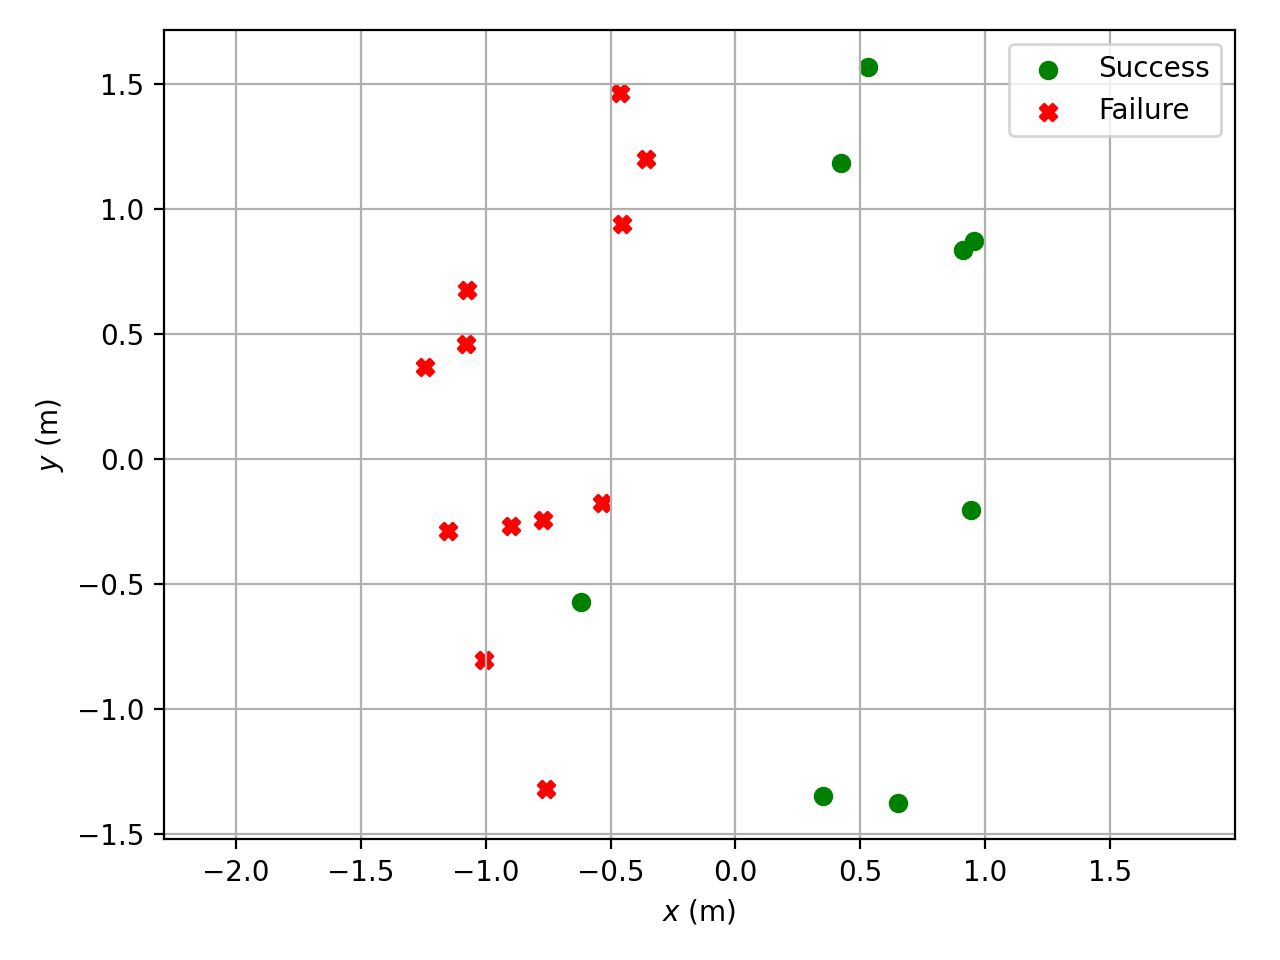
\includegraphics[width=0.85\textwidth]{pictures/Figure_1.png}
        	\caption{\textbf{Block Retrieval Response}}
        	\label{block_response}
        	\end{center}
        \end{figure}
        
        Investigating further into the data, filtering the information based on the sign of the x-coordinate revealed that block spawns in the positive x-direction were more successful than the in the negative x-direction. 
        
        % table for success rates
        \begin{table}[H]
            \begin{center}
            \setstretch{1}
            \caption{\textbf{Completion Rates Based on X Coordinate}}
            \label{table:completion}
            \begin{tabular}{|p{1.8in}|p{1.8in}|}
                \hline
                \textbf{Sign} & \textbf{Success Rate}\\ \hline
                 Positive & 100.0\%\\ \hline
                 Negative & 7.69\% \\ \hline
                 Total & 40\% \\ \hline
            \end{tabular}
            \end{center}
        \end{table}
        
        If the robot properly converged to the original spawn point, the errors were recorded and plotted in Figure \ref{fig:errorxy}. This characterizes the error build up in the x and y coordinates of the robot and demonstrates he inaccuracies in the controller even when the robot converges to its home location. The maximum magnitude of error demonstrated is about 0.053 m from the original spawn point. That is an non-negligible amount of error that should be accounted for.
        
        \begin{figure}[htp]
        	\begin{center}
        	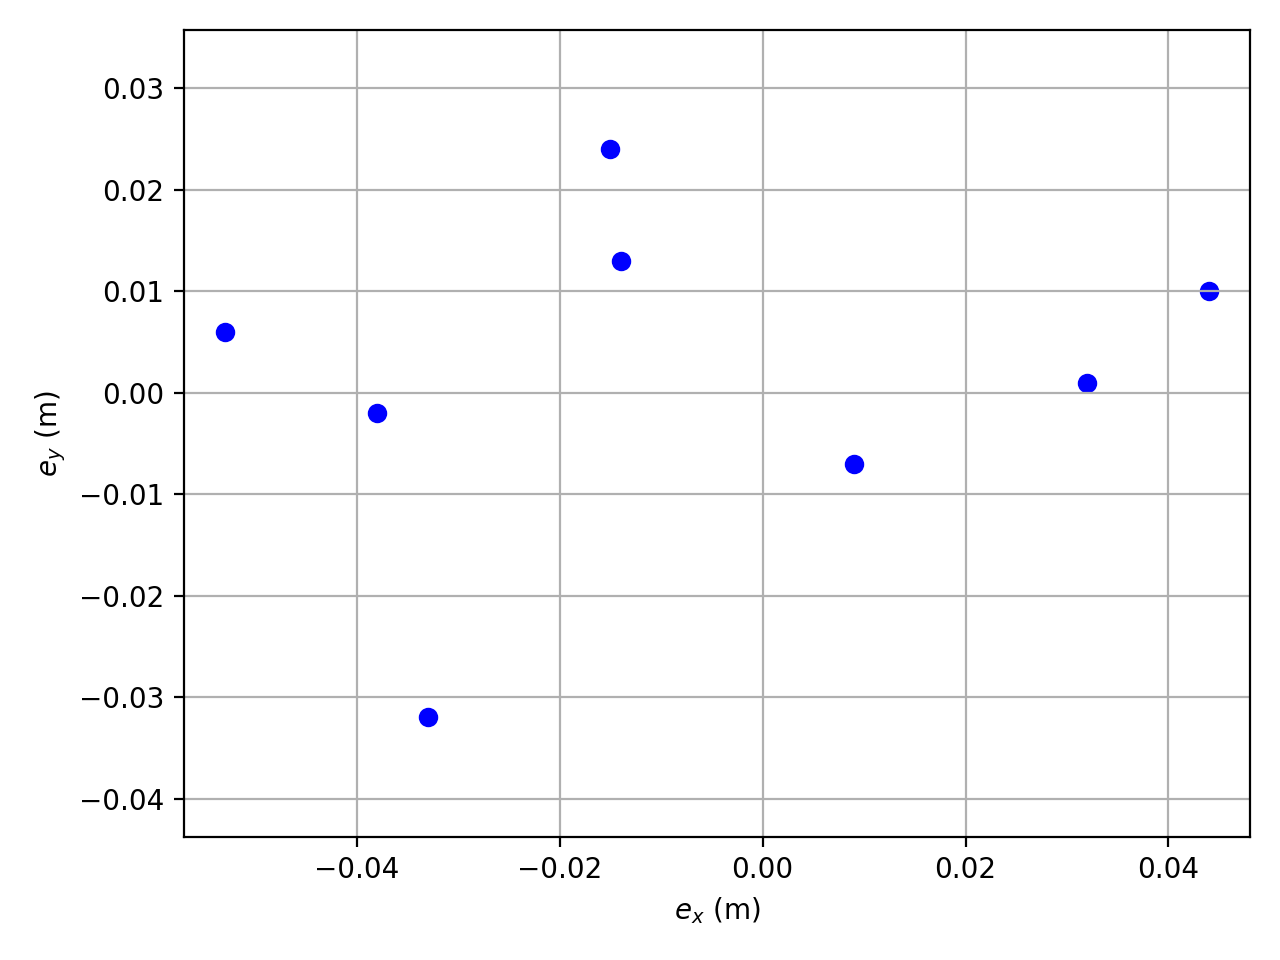
\includegraphics[width=0.8\textwidth]{pictures/Figure_2.png}
        	\caption{\textbf{Convergence Error}}
        	\label{fig:errorxy}
        	\end{center}
        \end{figure}
        
        Finally, looking into the gripping success rates, the team observed a very high success rate in converging towards the spawned block. This demonstrates the robot's ability to arrive at the desired location of block, and grip the block properly. 
        
        % table for gripping rate success
        \begin{table}[H]
            \begin{center}
            \setstretch{1}
            \caption{\textbf{Gripping Rates}}
            \label{table:gripping}
            \begin{tabular}{|p{1.8in}|p{1.8in}|}
                \hline
                \textbf{Success Rate} \\ \hline
                90\% \\ \hline
            \end{tabular}
            \end{center}
        \end{table}  
        
        Overall, the data demonstrates the ability to converge towards most blocks spawned within the task space of the robot, while the return back to its home location cannot be guaranteed. Furthermore, the program does not accurately return to the home position, characterized by the high level of error at the home location. 
    
    \subsection{Error Analysis} % Charlie 
    
        Out of these twenty trials, twelve were failures. All of the failures occurred when the block was spawned with a negative x-coordinate which points. Two of the failures were the result of a failure to grip the block, and in the remaining ten, the robot simply could not find a suitable location to drive to that would place the arm close enough to pick up the block. These results point to two possible sources of error: the motion planner and the camera.
        
        \subsubsection*{Returning Home}
            
            The main problem with the motion planner is the way it handles negative x-coordinates. The robot does not converge back to the spawn location when handling these values. Furthermore, even if the robot converges back to the home location successfully, there is a significant amount of error that could ruin the program. 
            
            Possible sources of error can be the automatically induced rotation of the robot. When the robot loads into the simulator, the robot is oriented correctly but with a slightly induced rotation on the block. This can be attributed to the inertial values of the cart interacting with the inertial values of the UR3 arm, inducing a rotation to disorient the cart. In the listing below, a clear rotation is induced, meaning these errors will build up over time and cause the system to fail. 
            
            \begin{quote} 
                \begin{lstlisting}[gobble=16,language=Python]
                twist: 
                  twist: 
                    linear: 
                      x: 1.78733181747e-05
                      y: 2.68657963054e-05
                      z: 0.0
                    angular: 
                      x: 0.0
                      y: 0.0
                      z: -5.13699727462e-05
                \end{lstlisting}
            \end{quote}
            
            These errors can be mitigated through further investigation of the simulated environment and interactions of the components. Another possible solution is to implement a better controller for this program to account for the error built-up from the induced rotation.
            
        \subsubsection*{Long-Distance Control}
        
            Another source of error is the camera. All of the calibration tests for the camera were run with blocks placed fairly close to the origin, meaning there was the possibility for a small amount of error being introduced that gets magnified as the blocks move further and further from the origin. Another larger possibility for error involves the assumptions made when running the camera calibration. It was assumed that there was no distortion in the camera's image as the distance from the origin increased. This was done to simplify the calibration, though it will cause some inaccuracies. In reality, there is increased distortion in the regions of the image further from the origin. Since the blob search function used in this project does not account for these distortions, it will calculate an incorrect spawn location for the block if the block is spawned far from the origin. 
            
            These errors can be mitigated through increased complexity of the CV software, accounting for these distortions. Additional cameras can be added as well to have multiple sources to more accurately sense the environment for the task space. An array of these cameras can determine which camera has the closest detection value to find the most accurate representation of the location of the block. 

\newpage
\section{Summary and Challenges} \label{sec:summary_challenges}
% acknowledge knap's team. 
    
    % Briefly summarize your project and what you found. Discuss what you learned, as well as some challenges you encountered (if any). Tell us what you would do differently if you were to attempt this project again and/or had more time.


    After a total of twenty tests, the team cannot say with confidence that GouBot is able to achieve its intended goals and bring happiness to the user. It demonstrated its ability to locate an object and return it to the origin in only a fraction of the trials that were run. In the process of bringing GouBot to life the team faced quite a few challenges that made the road difficult to navigate. The most difficult challenges involved modifying the UR3 gazebo files, getting the robot to move around in the task space, and working with Gazebo and Linux via virtual machine in general.
    
    As mentioned earlier, the \lstinline!.urdf!, \lstinline!.xacro!, and \lstinline!.launch! files provided to the team that were used to spawn and control the UR3 robot were very impressive. On one hand they were incredibly robust and helpful to use as a benchmark for what a gazebo simulation should look like. On the other hand, they were dense and complex which made them difficult to understand or modify. It took the team a substantial amount of time to figure out how to add a base vehicle to the robot, be it differential drive robot or translating prism. 
    
    Once the differential drive robot was attached to the bottom of the UR3, the team faced a lot of trouble using it to move the robot. There seemed to be something preventing the robot's movement because it was possible to change the velocity of the wheels and could observe them spinning. If these values were set to large values the robot would move a little bit, as if it were trying to move but something was holding it back. The team suspected that somewhere there was a physical interaction between the surface of the robot and the simulated world been created between the robot and the world. Though after multiple exhaustive searches through the code the source of the problem could not be located and ultimately the decision was made to swap out the differential drive robot in favor of a simpler solution.
    
    The robot was never able to be accurately controlled to a high level of reliability. The accuracy of the robot would significantly decrease over time, causing failure due to the induced rotation of the robot. For future work, it may be wise to implement a more complex controller to account for these changes, whether that be a modern or PID controller. 
    
    Another challenge the team faced was the fact that ROS and Gazebo could only run on Linux, which the team could only access through a virtual machine. This came with a significant drop in computer resources and meant that everything any team member tried to do took longer than it would have taken to do otherwise. Additionally, Gazebo would fail to launch a fairly frequently which added a significant amount of time to the data collection and testing process. For future work, it may be wise to utilize a simpler and more reliable simulation environment to interface with the controllers. 
    
    The team completed all of its goals of creating a robot to retrieve a randomly placed payload in this project. Along the way the team learned a lot about robotics, computer science, simulation technology and more. It was a great experience, and in the end it all came together as a resounding success in learning about robotics.
    
\section*{Acknowledgements}
    
    The team would like to thank Professor Driggs-Campbell and Professor Belabbas for their contribution in teaching the concepts required for this project. The team would like to thank their teaching assistant, Dhruv Mathur, for his contribution in teaching the practical applications for this project. Finally, the team would like to thank the iLuvRobotiks team for their help throughout this project \cite{iluvrobotiks}.

\printbibliography[
% heading=bibintoc,
title={References}
] 

\newpage

\end{document}